% =============================================================================
%  Machine Learning for Petroleum Engineers Using Python
%  Clase 3: pandas y Carga de Datos --- Producción y Well Logs (Volve)
%  SLB Ecuador | UDLA
%
%  Compilar: pdflatex -shell-escape presentacion.tex (x2 para refs)
% =============================================================================
\documentclass[aspectratio=169, 11pt]{beamer}

% ── Codificación y lenguaje ──────────────────────────────────────────────────
\usepackage[T1]{fontenc}
\usepackage[utf8]{inputenc}
\usepackage[spanish,es-noshorthands]{babel}

% ── Fuentes ──────────────────────────────────────────────────────────────────
\usepackage{FiraSans}
\usepackage{FiraMono}
\renewcommand{\familydefault}{\sfdefault}

% ── Gráficos y diagramas ────────────────────────────────────────────────────
\usepackage{graphicx}
\usepackage{tikz}
\usetikzlibrary{arrows.meta, positioning, shapes.geometric, calc, fit, decorations.pathreplacing}
\usepackage{fontawesome5}

% ── Código fuente ────────────────────────────────────────────────────────────
\usepackage{minted}
\usepackage{tcolorbox}
\tcbuselibrary{minted, skins, breakable}

% ── Tablas y utilidades ──────────────────────────────────────────────────────
\usepackage{amsmath}
\usepackage{colortbl}
\usepackage{booktabs}
\usepackage{multicol}
\usepackage{hyperref}
\usepackage{calc}

% =============================================================================
%  PALETA DE COLORES (rojo UDLA + variantes)
% =============================================================================
\definecolor{arcaRed}{HTML}{C82B40}
\definecolor{arcaDark}{HTML}{6B1525}
\definecolor{udlaCrimson}{HTML}{A31545}
\definecolor{arcaGray}{HTML}{F5F5F5}
\definecolor{arcaLightGray}{HTML}{EBEBEB}
\definecolor{textDark}{HTML}{2D2D2D}
\definecolor{textMuted}{HTML}{6B7280}
\definecolor{codeGreen}{HTML}{16A34A}
\definecolor{codeBlue}{HTML}{2563EB}
\definecolor{codeOrange}{HTML}{EA580C}
\definecolor{slbBlue}{HTML}{0014DC}
\definecolor{terminalBg}{HTML}{0F172A}
\definecolor{terminalGreen}{HTML}{86EFAC}
\definecolor{terminalMuted}{HTML}{94A3B8}
\definecolor{codeBg}{HTML}{FAFAFA}

% =============================================================================
%  CONFIGURACIÓN DEL TEMA BEAMER
% =============================================================================
\usetheme{default}
\usecolortheme{default}

\setbeamertemplate{navigation symbols}{}
\setbeamertemplate{footline}{}
\setbeamertemplate{headline}{}

\setbeamercolor{normal text}{fg=textDark}
\setbeamercolor{frametitle}{fg=arcaRed, bg=white}
\setbeamercolor{title}{fg=white}
\setbeamercolor{subtitle}{fg=white!85}
\setbeamercolor{author}{fg=white!80}
\setbeamercolor{date}{fg=white!70}
\setbeamercolor{item}{fg=arcaRed}
\setbeamercolor{subitem}{fg=arcaDark}
\setbeamercolor{block title}{fg=white, bg=arcaRed}
\setbeamercolor{block body}{fg=textDark, bg=arcaGray}
\setbeamercolor{block title alerted}{fg=white, bg=codeOrange}
\setbeamercolor{block body alerted}{fg=textDark, bg=arcaGray}
\setbeamercolor{block title example}{fg=white, bg=codeGreen}
\setbeamercolor{block body example}{fg=textDark, bg=arcaGray}
\setbeamercolor{section in toc}{fg=arcaDark}

\setbeamerfont{frametitle}{size=\Large, series=\bfseries}
\setbeamerfont{title}{size=\huge, series=\bfseries}
\setbeamerfont{subtitle}{size=\large}
\setbeamerfont{author}{size=\normalsize}
\setbeamerfont{date}{size=\small}
\setbeamerfont{block title}{size=\normalsize, series=\bfseries}
\setbeamerfont{footnote}{size=\tiny}

\setbeamertemplate{itemize item}{\scriptsize\raise1.5pt\hbox{\color{arcaRed}$\blacktriangleright$}}
\setbeamertemplate{itemize subitem}{\scriptsize\raise1pt\hbox{\color{arcaDark}$\bullet$}}
\setbeamertemplate{enumerate items}[default]
\setbeamercolor{enumerate item}{fg=arcaRed}

% =============================================================================
%  HEADER
% =============================================================================
\setbeamertemplate{headline}{%
  \begin{tikzpicture}[remember picture, overlay]
    \fill[arcaDark] (current page.north west) rectangle
      ([yshift=-0.7cm]current page.north east);
    \node[anchor=west, inner sep=0pt] at
      ([xshift=0.6cm, yshift=-0.35cm]current page.north west)
      {
\includegraphics[height=0.45cm]{../logo_udla_white.png}};
    \node[anchor=east, inner sep=0pt] at
      ([xshift=-0.6cm, yshift=-0.35cm]current page.north east)
      {
\includegraphics[height=0.42cm]{../SLB_white.png}};
  \end{tikzpicture}%
  \vspace{0.7cm}%
}

% =============================================================================
%  FOOTER
% =============================================================================
\setbeamertemplate{footline}{%
  \begin{tikzpicture}[remember picture, overlay]
    \draw[arcaLightGray, line width=0.4pt]
      ([yshift=0.55cm, xshift=0.6cm]current page.south west) --
      ([yshift=0.55cm, xshift=-0.6cm]current page.south east);
    \node[anchor=south, font=\tiny\color{textMuted}] at
      ([yshift=0.15cm]current page.south)
      {Machine Learning for Petroleum Engineers Using Python \(\cdot\) SLB Ecuador};
    \node[anchor=south east, font=\scriptsize\bfseries\color{arcaRed}] at
      ([xshift=-0.6cm, yshift=0.15cm]current page.south east)
      {\insertframenumber};
  \end{tikzpicture}%
}

% =============================================================================
%  FRAMETITLE personalizado con línea roja
% =============================================================================
\setbeamertemplate{frametitle}{%
  \vspace{0.25cm}%
  \usebeamerfont{frametitle}\usebeamercolor[fg]{frametitle}\insertframetitle%
  \par\vspace{2pt}%
  \begin{tikzpicture}
    \fill[arcaRed] (0,0) rectangle (3cm, 1.5pt);
    \fill[arcaLightGray] (3cm,0) rectangle (\textwidth, 0.5pt);
  \end{tikzpicture}%
  \vspace{0.1cm}%
}

% =============================================================================
%  ESTILO DE BLOQUES DE CÓDIGO (minted + tcolorbox)
% =============================================================================
\newtcblisting{pyblock}[1][]{%
  listing engine=minted,
  minted language=python,
  minted style=xcode,
  minted options={
    fontsize=\small,
    linenos=false,
    breaklines=true,
    python3=true
  },
  enhanced,
  colback=codeBg,
  colframe=arcaRed,
  left=8pt,
  right=6pt,
  top=5pt,
  bottom=5pt,
  boxrule=0pt,
  leftrule=3pt,
  arc=3pt,
  listing only,
  title={\hspace{-2pt}\faPython\hspace{5pt}Python},
  fonttitle=\scriptsize\bfseries,
  colbacktitle=arcaRed,
  coltitle=white,
  attach boxed title to top left={xshift=8pt, yshift=-7pt},
  boxed title style={
    arc=2pt, boxrule=0pt,
    top=1.5pt, bottom=1.5pt, left=6pt, right=6pt
  },
  drop fuzzy shadow=black!12,
  #1
}

\newtcblisting{outputblock}[1][]{%
  listing engine=minted,
  minted language=text,
  minted style=bw,
  minted options={
    fontsize=\small,
    breaklines=true,
    formatcom=\color{terminalGreen}
  },
  enhanced,
  colback=terminalBg,
  colframe=terminalBg,
  coltext=terminalGreen,
  left=10pt, right=6pt, top=5pt, bottom=5pt,
  boxrule=0pt,
  arc=3pt,
  listing only,
  title={\hspace{-2pt}\faTerminal\hspace{5pt}Output},
  fonttitle=\scriptsize\bfseries,
  colbacktitle=terminalGreen!85!black,
  coltitle=terminalBg,
  attach boxed title to top left={xshift=8pt, yshift=-7pt},
  boxed title style={
    arc=2pt, boxrule=0pt,
    top=1.5pt, bottom=1.5pt, left=6pt, right=6pt
  },
  #1
}

% =============================================================================
%  SECTION DIVIDERS
% =============================================================================
\newcommand{\sectionframe}[2]{%
  \begingroup
    \setbeamertemplate{headline}{}
    \setbeamertemplate{footline}{}
    \setbeamertemplate{navigation symbols}{}
    \begin{frame}[plain, noframenumbering]
      \begin{tikzpicture}[remember picture, overlay]
        \fill[arcaRed] (current page.south west) rectangle (current page.north east);
        \node[anchor=center, text=white, font=\Huge\bfseries, text width=12cm,
              align=center] at ([yshift=0.5cm]current page.center) {#1};
        \node[anchor=center, text=white!80, font=\large, text width=10cm,
              align=center] at ([yshift=-0.8cm]current page.center) {#2};
      \end{tikzpicture}
    \end{frame}
  \endgroup
}

% =============================================================================
%  METADATOS
% =============================================================================
\title{Machine Learning for Petroleum Engineers\\Using Python}
\subtitle{Módulo 3 · Clase 3: No Linealidad --- Árboles y Random Forest}
\author{Carlos Enrique Mosquera Trujillo}
\date{2026}

% =============================================================================
%  DOCUMENTO
% =============================================================================
% =============================================================================
%  DOCUMENTO
% =============================================================================
\begin{document}

% ── PORTADA ──────────────────────────────────────────────────────────────────
{
\setbeamertemplate{headline}{}
\setbeamertemplate{footline}{}
\begin{frame}[plain, noframenumbering]
  \begin{tikzpicture}[remember picture, overlay]
    \fill[white] (current page.south west) rectangle (current page.north east);
    \fill[arcaRed] (current page.north west) rectangle ([yshift=-0.35cm]current page.north east);
    \fill[arcaDark] (current page.south west) rectangle ([yshift=0.35cm]current page.south east);
    \fill[arcaRed]
      ([xshift=1.1cm, yshift=-0.35cm]current page.north west) rectangle
      ([xshift=1.15cm, yshift=0.35cm]current page.south west);
    \node[anchor=north west, inner sep=0pt] at
      ([xshift=1.8cm, yshift=-1.2cm]current page.north west)
      {
\includegraphics[height=1.6cm]{../logo_udla.png}};
    \node[anchor=north east, inner sep=0pt] at
      ([xshift=-1.5cm, yshift=-1.2cm]current page.north east)
      {
\includegraphics[height=1.5cm]{../SLB.png}};
    \node[anchor=center, text=arcaDark, text width=14.5cm, align=center] at
      ([yshift=0.95cm]current page.center) {
        {\LARGE\bfseries Machine Learning for Petroleum Engineers}\\[8pt]
        {\LARGE\bfseries Using Python}
      };
    \fill[arcaRed]
      ([yshift=-0.35cm, xshift=-3.2cm]current page.center) rectangle
      ([yshift=-0.28cm, xshift=3.2cm]current page.center);
    \node[anchor=center, text=arcaRed, font=\large, text width=13cm, align=center] at
      ([yshift=-1.3cm]current page.center) {
        Módulo 3 · Clase 3\\[3pt]
        No Linealidad: Árboles de Decisión y Random Forest
      };
    \node[anchor=center, text=textMuted, font=\normalsize] at
      ([yshift=-2.5cm]current page.center) {
        {\color{arcaRed}\faUser}\hspace{6pt}Carlos Enrique Mosquera Trujillo
        \hspace{16pt}
        {\color{arcaRed}\faIndustry}\hspace{4pt}SLB Ecuador
      };
  \end{tikzpicture}
\end{frame}
}

% ── RECAP + RUTA ─────────────────────────────────────────────────────────────
\begin{frame}[shrink=8]{Dónde Estamos}
  \vspace{-4pt}
  \begin{columns}[T]
    \begin{column}{0.48\textwidth}
      {\small\color{arcaDark}\bfseries\faCheckCircle\hspace{5pt}Ya tenemos:}
      \vspace{4pt}
      {\footnotesize\color{textMuted}
      \begin{itemize}\setlength{\itemsep}{3pt}
        \item[{\color{codeGreen}\scriptsize\faCheck}]
          Regresión lineal: predecir un \textbf{número}
        \item[{\color{codeGreen}\scriptsize\faCheck}]
          Regresión logística: predecir una \textbf{etiqueta}
        \item[{\color{codeGreen}\scriptsize\faCheck}]
          Métricas + \textbf{costo de negocio} y umbral
        \item[{\color{codeGreen}\scriptsize\faCheck}]
          Train/test, estandarización, binarización
      \end{itemize}
      }
      \vspace{6pt}
      {\scriptsize\color{textMuted}\itshape
        Pero ambos modelos comparten un límite:
        por dentro son \textbf{una recta}.}
    \end{column}
    \begin{column}{0.48\textwidth}
      {\small\color{arcaDark}\bfseries\faForward\hspace{5pt}Hoy:}
      \vspace{4pt}
      {\footnotesize\color{textMuted}
      \begin{itemize}\setlength{\itemsep}{3pt}
        \item[{\color{arcaRed}\scriptsize\faArrowRight}]
          Qué es la \textbf{no linealidad} y por qué el mundo
          real casi siempre es así
        \item[{\color{arcaRed}\scriptsize\faArrowRight}]
          Ver a la recta \textbf{fracasar} (las lunas)
        \item[{\color{arcaRed}\scriptsize\faArrowRight}]
          \textbf{Árboles de decisión}, explicados desde cero
        \item[{\color{arcaRed}\scriptsize\faStar}]
          \textbf{Random Forest} --- y batir el récord de costo
          de la Clase 2
      \end{itemize}
      }
      \vspace{4pt}
      {\scriptsize\color{arcaDark}\itshape
        Al final: los árboles también predicen números
        (un \textbf{medidor virtual de flujo}).}
    \end{column}
  \end{columns}
\end{frame}

% ═════════════════════════════════════════════════════════════════════════════
\sectionframe{¿Qué es la No Linealidad?}{Cuando el paso deja de ser parejo}
% ═════════════════════════════════════════════════════════════════════════════

% ── RECAP LINEAL ─────────────────────────────────────────────────────────────
\begin{frame}[shrink=10]{Recuerden: Lineal = el Paso Parejo}
  \vspace{-4pt}
  {\small\color{arcaDark}\bfseries
    En la Clase 1 lo definimos: lineal es cuando el mismo paso en X produce \textbf{siempre el mismo} paso en Y.}

  \vspace{8pt}
  \begin{columns}[T]
    \begin{column}{0.48\textwidth}
      \begin{tcolorbox}[colback=arcaGray, colframe=codeGreen, boxrule=0pt, leftrule=3pt,
        arc=3pt, left=6pt, right=6pt, top=5pt, bottom=5pt]
        {\scriptsize\color{codeGreen}\bfseries\faCheck\hspace{4pt}LINEAL (el paso vale igual)}\\[4pt]
        {\scriptsize\color{textMuted}
          Tanquear el carro: el galón 1 cuesta lo mismo
          que el galón 10.\\[3pt]
          Presión hidrostática: cada 100 m suman
          \(\approx\) lo mismo.}
      \end{tcolorbox}
    \end{column}
    \begin{column}{0.48\textwidth}
      \begin{tcolorbox}[colback=arcaGray, colframe=arcaRed, boxrule=0pt, leftrule=3pt,
        arc=3pt, left=6pt, right=6pt, top=5pt, bottom=5pt]
        {\scriptsize\color{arcaRed}\bfseries\faTimes\hspace{4pt}NO LINEAL (el paso cambia)}\\[4pt]
        {\scriptsize\color{textMuted}
          Abrir el choke de 20\,\% a 30\,\% \textbf{no} da lo
          mismo que de 70\,\% a 80\,\%.\\[3pt]
          El declive: el primer año el pozo cae muchísimo;
          el quinto, casi nada.}
      \end{tcolorbox}
    \end{column}
  \end{columns}

  \vspace{10pt}
  {\footnotesize\color{textMuted}
  \begin{itemize}\setlength{\itemsep}{4pt}
    \item[{\color{arcaRed}\scriptsize\faArrowRight}]
      \textbf{No lineal} = el efecto de una variable \textbf{depende de dónde estás}.
    \item[{\color{arcaRed}\scriptsize\faArrowRight}]
      Y a veces depende de \textbf{otra} variable: eso se llama \textbf{interacción}
      (el efecto del choke depende de la presión disponible).
  \end{itemize}
  }
\end{frame}

% ── EJEMPLOS DE CAMPO ────────────────────────────────────────────────────────
\begin{frame}[shrink=18]{El Mundo Real Rara Vez es una Recta}
  \vspace{-4pt}
  {\small\color{arcaDark}\bfseries
    Piensen en su operación: ¿cuántas de estas relaciones son ``parejas''?}

  \vspace{6pt}
  \centering
  {\footnotesize
  \renewcommand{\arraystretch}{1.5}
  \begin{tabular}{@{}p{4.6cm} p{6.8cm}@{}}
    \toprule
    {\bfseries\color{arcaDark} Relación} & {\bfseries\color{arcaRed} Por qué NO es lineal} \\
    \midrule
    \rowcolor{arcaGray}
    Choke vs caudal & al inicio cada punto de apertura suma mucho; cerca del máximo, casi nada \\
    Tiempo vs producción & la curva de declive: cae rápido y luego lento \\
    \rowcolor{arcaGray}
    Frecuencia de bomba vs caudal & sube hasta una \textbf{meseta}: el pozo no da más \\
    Presión vs caudal (IPR) & la curva IPR es\ldots{} una \textbf{curva} \\
    \rowcolor{arcaGray}
    Temperatura vs viscosidad & exponencial: unos grados cambian todo \\
    GR vs litología & no es gradual: hay un \textbf{umbral} donde la roca cambia \\
    \bottomrule
  \end{tabular}
  }

  \vspace{8pt}
  {\footnotesize\color{textMuted}
    \faLightbulb[regular]\hspace{4pt}%
    La recta es el modelo \textbf{más simple y explicable} --- por eso empezamos ahí.
    Pero cuando la física es curva, \textbf{necesitamos modelos que doblen}.}
\end{frame}

% ── LAS LUNAS ────────────────────────────────────────────────────────────────
\begin{frame}{Un Experimento: las Dos Lunas}
  \vspace{-6pt}
  {\small\color{arcaDark}\bfseries
    Un problema de juguete, diseñado para \textbf{ver} el límite de la recta.}

  \vspace{4pt}
  \begin{columns}[T]
    \begin{column}{0.52\textwidth}
      \centering
      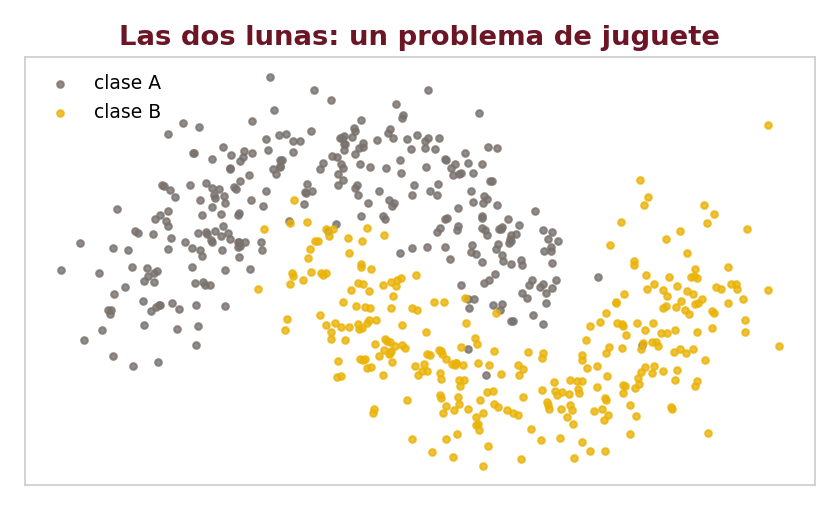
\includegraphics[width=0.94\textwidth]{fig_lunas.png}
    \end{column}
    \begin{column}{0.44\textwidth}
      {\footnotesize\color{textMuted}
      \begin{itemize}\setlength{\itemsep}{6pt}
        \item[{\color{arcaRed}\scriptsize\faArrowRight}]
          Dos grupos con forma de \textbf{medialunas
          entrelazadas}.
        \item[{\color{arcaRed}\scriptsize\faEye}]
          Cualquier persona los separa \textbf{a ojo},
          sin pensar.
        \item[{\color{arcaRed}\scriptsize\faQuestion}]
          Pregunta: ¿puede separarlos una \textbf{línea
          recta}?
      \end{itemize}
      }
      \vspace{4pt}
      {\scriptsize\color{arcaDark}\itshape
        Este dataset (\texttt{make\_moons}) es el examen
        clásico de no linealidad en ML.}
    \end{column}
  \end{columns}
\end{frame}

% ── LOGÍSTICA FRACASA ────────────────────────────────────────────────────────
\begin{frame}{La Regresión Logística lo Intenta\ldots{} y Fracasa}
  \vspace{-6pt}
  {\small\color{arcaDark}\bfseries
    La logística solo sabe trazar una \textbf{frontera recta}. Es lo mejor que puede hacer:}

  \vspace{4pt}
  \begin{columns}[T]
    \begin{column}{0.54\textwidth}
      \centering
      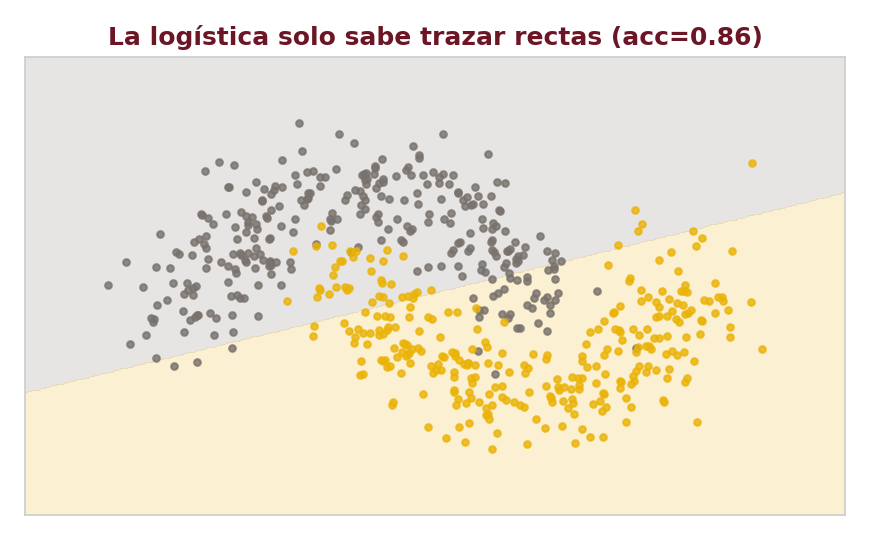
\includegraphics[width=\textwidth]{fig_lunas_logistica.png}
    \end{column}
    \begin{column}{0.42\textwidth}
      {\footnotesize\color{textMuted}
      \begin{itemize}\setlength{\itemsep}{6pt}
        \item[{\color{arcaRed}\scriptsize\faTimes}]
          Su recta corta las dos lunas por la mitad:
          se queda en \textbf{0.86} \textbf{para siempre}.
        \item[{\color{arcaRed}\scriptsize\faArrowRight}]
          No es falta de datos ni de ajuste: es un límite
          \textbf{estructural}. La recta no puede doblar.
        \item[{\color{arcaRed}\scriptsize\faQuestion}]
          ¿Qué modelo puede seguir la forma de las lunas?
          Eso construiremos hoy, \textbf{paso a paso}.
      \end{itemize}
      }
    \end{column}
  \end{columns}
\end{frame}

% ═════════════════════════════════════════════════════════════════════════════
\sectionframe{El Reto de Hoy}{Batir el récord de la Clase 2}
% ═════════════════════════════════════════════════════════════════════════════

% ── VOLVER A LA LITOLOGÍA ────────────────────────────────────────────────────
\begin{frame}[shrink=8]{Volvemos a la Litología --- a Propósito}
  \vspace{-4pt}
  {\small\color{arcaDark}\bfseries
    Mismo problema de la Clase 2: ¿esta roca es \textbf{reservorio} (arenisca) o \textbf{sello} (lutita)?}

  \vspace{6pt}
  \begin{columns}[T]
    \begin{column}{0.50\textwidth}
      {\footnotesize\color{textMuted}
      \begin{itemize}\setlength{\itemsep}{6pt}
        \item[{\color{arcaRed}\scriptsize\faDatabase}]
          Mismo dataset FORCE 2020: \textbf{62\,792} profundidades,
          11 pozos, 5 registros.
        \item[{\color{arcaRed}\scriptsize\faBalanceScale}]
          Mismo desbalance: \textbf{83\,\% lutita}, 17\,\% arenisca.
        \item[{\color{codeGreen}\scriptsize\faCheck}]
          ¿Por qué repetirlo? Para una comparación
          \textbf{justa}: mismos datos, mismo test, mismas
          métricas. \textbf{Solo cambia el modelo.}
      \end{itemize}
      }
    \end{column}
    \begin{column}{0.46\textwidth}
      \begin{tcolorbox}[colback=arcaGray, colframe=arcaRed, boxrule=0pt, leftrule=3pt,
        arc=3pt, left=6pt, right=6pt, top=5pt, bottom=5pt]
        {\scriptsize\color{arcaDark}\bfseries El récord a batir (Clase 2):}\\[5pt]
        {\scriptsize\color{textMuted}
          Regresión logística, umbral 0.5:\\[2pt]
          \(\bullet\) accuracy \textbf{0.944}\\
          \(\bullet\) recall \textbf{0.79} (se escapan 2 de cada 10 zonas)\\
          \(\bullet\) \textbf{563 zonas perdidas}, 323 cañoneos en seco\\
          \(\bullet\) costo total: \textbf{5\,953}}
      \end{tcolorbox}
      \vspace{4pt}
      {\scriptsize\color{arcaDark}\itshape
        La física de la litología tiene \textbf{umbrales}
        e \textbf{interacciones}: terreno ideal para
        modelos no lineales.}
    \end{column}
  \end{columns}
\end{frame}

% ═════════════════════════════════════════════════════════════════════════════
\sectionframe{Árboles de Decisión}{Desde cero, paso a paso}
% ═════════════════════════════════════════════════════════════════════════════

% ── QUÉ ES (CONCEPTO PURO) ───────────────────────────────────────────────────
\begin{frame}[shrink=12]{¿Qué es un Árbol de Decisión? (Sin Datos Todavía)}
  \vspace{-6pt}
  {\small\color{arcaDark}\bfseries
    Es la forma en que \textbf{ya deciden} en el campo: una cadena de preguntas de sí/no.}

  \vspace{8pt}
  \centering
  \begin{tikzpicture}[
    preg/.style={rectangle, rounded corners=5pt, fill=arcaGray, draw=arcaRed,
      line width=1pt, minimum width=3.6cm, minimum height=0.85cm, align=center,
      font=\scriptsize, text=textDark},
    hoja/.style={rectangle, rounded corners=5pt, minimum width=2.6cm,
      minimum height=0.75cm, align=center, font=\scriptsize\bfseries, text=white},
    ar/.style={-{Stealth[length=5pt]}, line width=1.1pt, textMuted},
    lb/.style={font=\tiny\color{textMuted}, fill=white, inner sep=1pt}]
    \node[preg] (q1) {¿La bomba vibra más\\de lo normal?};
    \node[hoja, fill=codeGreen!85!black, below left=0.7cm and 1.6cm of q1] (h1) {seguir operando};
    \node[preg, below right=0.7cm and 1.0cm of q1] (q2) {¿La temperatura del\\motor supera 90\(^{\circ}\)C?};
    \node[hoja, fill=codeOrange, below left=0.7cm and 0.6cm of q2] (h2) {programar revisión};
    \node[hoja, fill=arcaRed, below right=0.7cm and 0.4cm of q2] (h3) {PARAR la bomba};
    \draw[ar] (q1) -- (h1) node[lb, midway, above left] {no};
    \draw[ar] (q1) -- (q2) node[lb, midway, above right] {sí};
    \draw[ar] (q2) -- (h2) node[lb, midway, above left] {no};
    \draw[ar] (q2) -- (h3) node[lb, midway, above right] {sí};
  \end{tikzpicture}

  \vspace{10pt}
  {\footnotesize\color{textMuted}
  \begin{itemize}\setlength{\itemsep}{3pt}
    \item[{\color{arcaRed}\scriptsize\faArrowRight}]
      Cada pregunta \textbf{divide} los casos en dos; al final de cada camino
      hay una \textbf{decisión}.
    \item[{\color{codeGreen}\scriptsize\faCheck}]
      Así opera un supervisor con 20 años de experiencia. El árbol de ML
      hace \textbf{exactamente esto}.
  \end{itemize}
  }
\end{frame}

% ── ANATOMÍA ─────────────────────────────────────────────────────────────────
\begin{frame}[shrink=15]{La Anatomía: Raíz, Ramas y Hojas}
  \vspace{-6pt}
  {\small\color{arcaDark}\bfseries
    El mismo diagrama, con los nombres técnicos que usaremos el resto de la clase.}

  \vspace{8pt}
  \centering
  \begin{tikzpicture}[
    preg/.style={rectangle, rounded corners=5pt, fill=arcaGray, draw=arcaRed,
      line width=1pt, minimum width=3.4cm, minimum height=0.8cm, align=center,
      font=\scriptsize, text=textDark},
    hoja/.style={rectangle, rounded corners=5pt, minimum width=2.4cm,
      minimum height=0.7cm, align=center, font=\scriptsize\bfseries, text=white},
    ar/.style={-{Stealth[length=5pt]}, line width=1.1pt, textMuted},
    tag/.style={font=\tiny\bfseries\color{arcaRed}, align=left}]
    \node[preg] (q1) {pregunta 1};
    \node[hoja, fill=codeGreen!85!black, below left=0.65cm and 1.5cm of q1] (h1) {decisión A};
    \node[preg, below right=0.65cm and 0.9cm of q1] (q2) {pregunta 2};
    \node[hoja, fill=codeOrange, below left=0.65cm and 0.5cm of q2] (h2) {decisión B};
    \node[hoja, fill=arcaRed, below right=0.65cm and 0.3cm of q2] (h3) {decisión C};
    \draw[ar] (q1) -- (h1); \draw[ar] (q1) -- (q2);
    \draw[ar] (q2) -- (h2); \draw[ar] (q2) -- (h3);
    % etiquetas
    \node[tag, left=1.1cm of q1] (t1) {NODO RAÍZ\\{\tiny la primera pregunta,}\\{\tiny la más importante}};
    \draw[-{Stealth[length=4pt]}, arcaRed!60] (t1) -- (q1);
    \node[tag, right=1.6cm of q2] (t2) {PROFUNDIDAD\\{\tiny cuántos niveles}\\{\tiny de preguntas}};
    \node[tag, below=0.5cm of h2] (t3) {HOJAS\\{\tiny donde termina el camino:}\\{\tiny la predicción}};
    \draw[-{Stealth[length=4pt]}, arcaRed!60] (t3) -- (h2);
  \end{tikzpicture}

  \vspace{8pt}
  {\footnotesize\color{textMuted}
    \faLightbulb[regular]\hspace{4pt}%
    Este árbol tiene \textbf{profundidad 2}: máximo dos preguntas antes de decidir.
    Recuerden esa palabra --- será \textbf{la perilla clave} del modelo.}
\end{frame}

% ── USTEDES YA PIENSAN EN ÁRBOLES ────────────────────────────────────────────
\begin{frame}[shrink=8]{Ustedes Ya Piensan en Árboles (con Datos)}
  \vspace{-4pt}
  {\small\color{arcaDark}\bfseries
    En petrofísica, esas preguntas de sí/no tienen nombre: \textbf{cutoffs}.}

  \vspace{8pt}
  \begin{columns}[T]
    \begin{column}{0.48\textwidth}
      {\footnotesize\color{textMuted}
      \begin{itemize}\setlength{\itemsep}{7pt}
        \item[{\color{arcaRed}\scriptsize\faCodeBranch}]
          ``Si el \texttt{GR} \(<\) 60 \(\to\) arena; si no \(\to\) arcilla.''
        \item[{\color{arcaRed}\scriptsize\faCodeBranch}]
          Y los encadenan: ``si es arena \textbf{y} la porosidad
          \(>\) 15\,\% \textbf{y} la resistividad es alta
          \(\to\) zona de interés.''
        \item[{\color{arcaRed}\scriptsize\faQuestion}]
          Pero\ldots{} ¿por qué 60 y no 55? ¿Por qué GR primero
          y no la porosidad?
      \end{itemize}
      }
    \end{column}
    \begin{column}{0.48\textwidth}
      \begin{tcolorbox}[colback=arcaGray, colframe=arcaRed, boxrule=0pt, leftrule=3pt,
        arc=3pt, left=6pt, right=6pt, top=5pt, bottom=5pt]
        {\scriptsize\color{arcaDark}\bfseries La diferencia con el árbol de ML:}\\[4pt]
        {\scriptsize\color{textMuted}
          los cutoffs del intérprete salen de la
          \textbf{experiencia}. Los del árbol salen de
          \textbf{probar todos los cortes posibles en los
          datos} y quedarse con los que mejor separan.\\[4pt]
          Ni mejor ni peor: \textbf{verificable y repetible}.}
      \end{tcolorbox}
    \end{column}
  \end{columns}

  \vspace{8pt}
  \centering
  {\footnotesize\color{arcaDark}
    Veamos exactamente \textbf{cómo elige} la máquina un corte.}
\end{frame}

% ── CÓMO ELIGE LA MÁQUINA ────────────────────────────────────────────────────
\begin{frame}[shrink=8]{¿Cómo Elige la Máquina la Pregunta?}
  \vspace{-4pt}
  {\small\color{arcaDark}\bfseries
    Fuerza bruta inteligente: prueba \textbf{todos} los cortes de \textbf{todas} las variables.}

  \vspace{8pt}
  {\footnotesize\color{textMuted}
  \begin{enumerate}\setlength{\itemsep}{8pt}
    \item[{\color{arcaRed}\bfseries 1.}]
      Toma una variable (p.\ ej.\ \texttt{GR}) y un corte candidato (p.\ ej.\ 55):
      divide los datos en dos grupos.
    \item[{\color{arcaRed}\bfseries 2.}]
      Mide qué tan \textbf{puros} quedaron los grupos: un grupo es puro si
      casi todos sus puntos son de la \textbf{misma clase}.
    \item[{\color{arcaRed}\bfseries 3.}]
      Repite con \textbf{cada corte posible de cada variable} y se queda con
      el que deja los grupos \textbf{más puros}.
    \item[{\color{arcaRed}\bfseries 4.}]
      Dentro de cada grupo, \textbf{vuelve a empezar}: busca la mejor pregunta
      para ese subgrupo. Así crece el árbol.
  \end{enumerate}
  }

  \vspace{8pt}
  {\footnotesize\color{textMuted}
    \faLightbulb[regular]\hspace{4pt}%
    ``Puro'' es la versión formal de lo que un intérprete busca a ojo:
    un corte donde \textbf{a un lado quede la arena y al otro la arcilla}.}
\end{frame}

% ── EL PRIMER CORTE REAL ─────────────────────────────────────────────────────
\begin{frame}{El Primer Corte, con Nuestros Datos Reales}
  \vspace{-6pt}
  {\small\color{arcaDark}\bfseries
    Dejamos que la máquina elija \textbf{una sola pregunta} sobre el \texttt{GR}. Esto encontró:}

  \vspace{4pt}
  \begin{columns}[T]
    \begin{column}{0.56\textwidth}
      \centering
      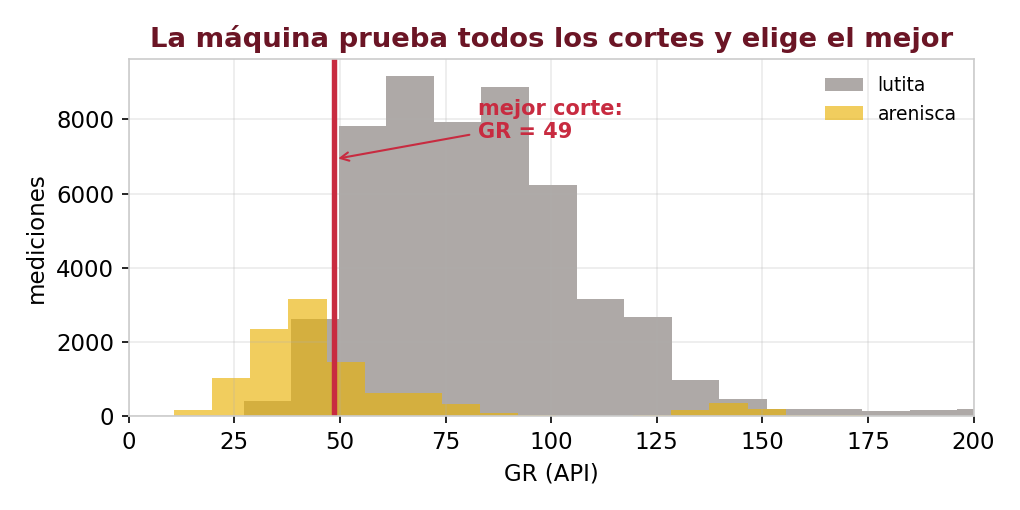
\includegraphics[width=\textwidth]{fig_corte_gr.png}
    \end{column}
    \begin{column}{0.40\textwidth}
      {\footnotesize\color{textMuted}
      \begin{itemize}\setlength{\itemsep}{6pt}
        \item[{\color{codeGreen}\scriptsize\faCheck}]
          El corte óptimo: \textbf{GR = 49}. Muy cerca del
          cutoff que un intérprete usaría (\(\sim\)50--60).
        \item[{\color{codeGreen}\scriptsize\faCheck}]
          Con \textbf{una sola pregunta}: accuracy
          \textbf{0.90} --- ya le gana al ``modelo tonto''
          (0.83).
        \item[{\color{arcaRed}\scriptsize\faArrowRight}]
          Pero el traslape no se resuelve con un corte:
          hay que \textbf{seguir preguntando}.
      \end{itemize}
      }
    \end{column}
  \end{columns}
\end{frame}

% ── EL ÁRBOL REAL ────────────────────────────────────────────────────────────
\begin{frame}[shrink=8]{Encadenando Preguntas: el Árbol Crece}
  \vspace{-4pt}
  {\small\color{arcaDark}\bfseries
    Con profundidad 2, la máquina eligió esto. Leámoslo juntos, nodo por nodo.}

  \vspace{2pt}
  \centering
  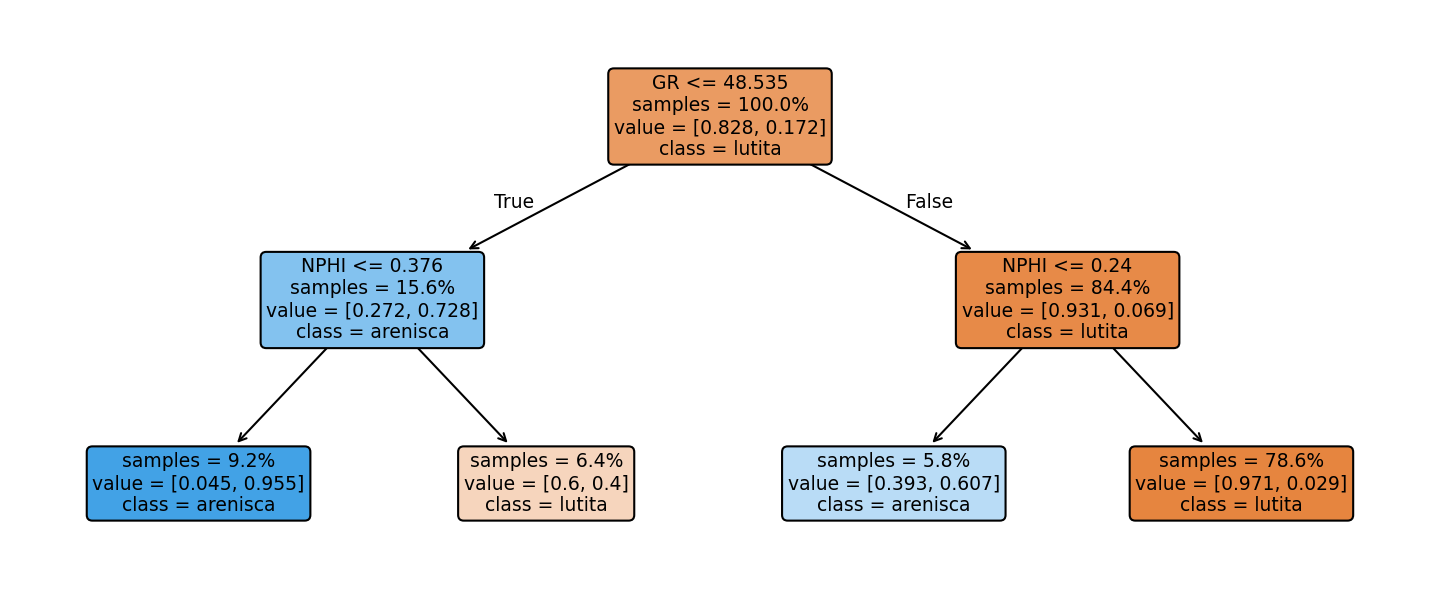
\includegraphics[width=0.86\textwidth]{fig_arbol_diagrama.png}

  \vspace{4pt}
  {\footnotesize\color{textMuted}
  \begin{itemize}\setlength{\itemsep}{2pt}
    \item[{\color{arcaRed}\scriptsize\faArrowRight}]
      \textbf{Raíz}: ¿GR \(\leq\) 49? --- la misma pregunta de la slide anterior.
    \item[{\color{arcaRed}\scriptsize\faArrowRight}]
      Luego refina con \texttt{NPHI} (la porosidad de neutrón) \textbf{en ambos lados},
      con cortes \textbf{distintos} en cada lado.
    \item[{\color{codeGreen}\scriptsize\faCheck}]
      GR bajo + NPHI bajo \(\to\) \textbf{arenisca}. GR alto \(\to\) \textbf{lutita}.
      La física, aprendida de los datos.
  \end{itemize}
  }
\end{frame}

% ── LAS LUNAS RESUELTAS ──────────────────────────────────────────────────────
\begin{frame}{Ahora Sí: las Lunas con un Árbol}
  \vspace{-6pt}
  {\small\color{arcaDark}\bfseries
    Cada pregunta corta el plano en dos. Muchas preguntas = una frontera de \textbf{escalones}.}

  \vspace{4pt}
  \begin{columns}[T]
    \begin{column}{0.54\textwidth}
      \centering
      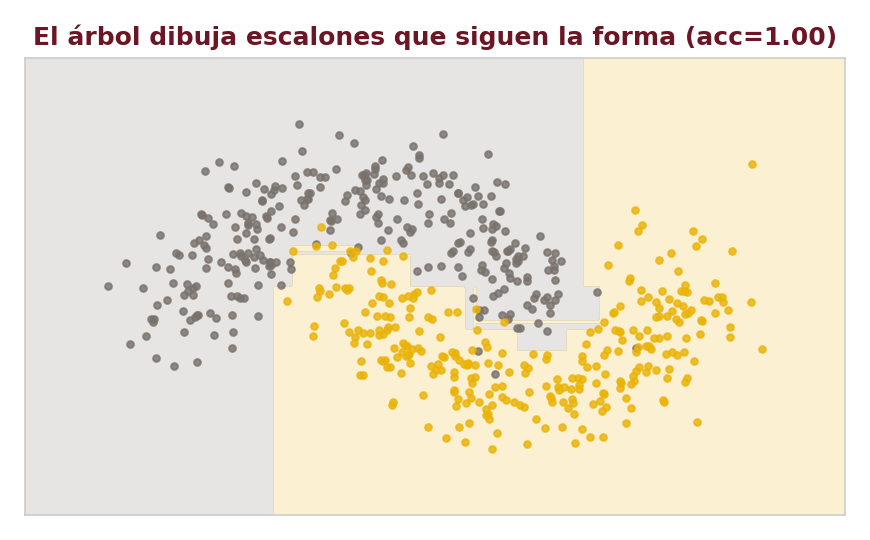
\includegraphics[width=\textwidth]{fig_lunas_arbol.png}
    \end{column}
    \begin{column}{0.42\textwidth}
      {\footnotesize\color{textMuted}
      \begin{itemize}\setlength{\itemsep}{6pt}
        \item[{\color{codeGreen}\scriptsize\faCheck}]
          Los escalones \textbf{siguen la forma} de las lunas:
          accuracy \textbf{1.00} donde la recta se quedó
          en 0.86.
        \item[{\color{arcaRed}\scriptsize\faArrowRight}]
          El árbol nunca ``dobla'' --- pero acumula tantos
          cortes rectos que \textbf{aproxima cualquier
          frontera}.
        \item[{\color{arcaRed}\scriptsize\faArrowRight}]
          Igual que los escalones aproximaban la curva
          del declive.
      \end{itemize}
      }
    \end{column}
  \end{columns}
\end{frame}

% ── EN CÓDIGO ────────────────────────────────────────────────────────────────
\begin{frame}[fragile,shrink=25]{En Código: el Mismo Patrón de Siempre}
  \vspace{-4pt}
  {\small\color{arcaDark}\bfseries
    Cambia el modelo, no el flujo. Y un regalo: los árboles \textbf{no necesitan estandarización}.}

  \vspace{4pt}
  \begin{columns}[T]
    \begin{column}{0.54\textwidth}
      \begin{pyblock}
from sklearn.tree import DecisionTreeClassifier

arbol = DecisionTreeClassifier(
    max_depth=5, random_state=42)
arbol.fit(X_tr, y_tr)

print(arbol.score(X_te, y_te))
      \end{pyblock}
      \vspace{2pt}
      \begin{outputblock}
0.957
      \end{outputblock}
    \end{column}
    \begin{column}{0.42\textwidth}
      {\scriptsize\color{textMuted}
      \begin{itemize}\setlength{\itemsep}{5pt}
        \item[{\color{codeGreen}\scriptsize\faCheck}]
          Con 5 niveles: accuracy \textbf{0.957}, recall
          \textbf{0.84} --- ya supera a la logística
          (0.944 / 0.79).
        \item[{\color{arcaRed}\scriptsize\faArrowRight}]
          \texttt{max\_depth}: cuántos niveles de preguntas.
          \textbf{La perilla clave.}
        \item[{\color{arcaRed}\scriptsize\faArrowRight}]
          Los cortes comparan cada variable \textbf{consigo
          misma} \(\to\) las escalas no importan.
      \end{itemize}
      }
    \end{column}
  \end{columns}
\end{frame}

% ── OVERFITTING ──────────────────────────────────────────────────────────────
\begin{frame}{La Tentación: ¿y si lo Dejamos Crecer sin Límite?}
  \vspace{-6pt}
  {\small\color{arcaDark}\bfseries
    Más profundidad = más poder\ldots{} hasta que empieza a \textbf{memorizar}.}

  \vspace{4pt}
  \begin{columns}[T]
    \begin{column}{0.56\textwidth}
      \centering
      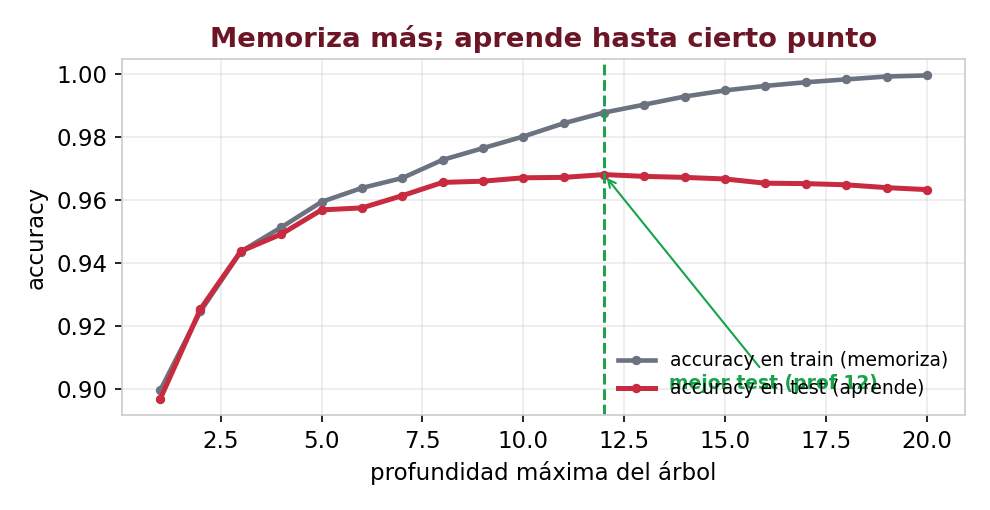
\includegraphics[width=\textwidth]{fig_overfit.png}
    \end{column}
    \begin{column}{0.40\textwidth}
      {\footnotesize\color{textMuted}
      \begin{itemize}\setlength{\itemsep}{5pt}
        \item[{\color{arcaRed}\scriptsize\faArrowRight}]
          Sin límite, el árbol crea una hoja para
          \textbf{cada rincón} de los datos: accuracy
          \textbf{train = 1.000}.
        \item[{\color{arcaRed}\scriptsize\faExclamationTriangle}]
          Pero en \textbf{test} deja de mejorar: aprendió
          el \textbf{ruido}, no el patrón.
        \item[{\color{codeGreen}\scriptsize\faCheck}]
          Es el \textbf{overfitting} de la Clase 1, ahora
          \textbf{visible en una curva}.
      \end{itemize}
      }
    \end{column}
  \end{columns}
\end{frame}

% ── EL ÁRBOL SOLO ES FRÁGIL ──────────────────────────────────────────────────
\begin{frame}[shrink=8]{El Árbol Solo: Poderoso pero Indisciplinado}
  \vspace{-4pt}
  {\small\color{arcaDark}\bfseries
    Dos debilidades que impiden confiar en un único árbol.}

  \vspace{8pt}
  \begin{columns}[T]
    \begin{column}{0.48\textwidth}
      \begin{tcolorbox}[colback=arcaGray, colframe=arcaRed, boxrule=0pt, leftrule=3pt,
        arc=3pt, left=6pt, right=6pt, top=5pt, bottom=5pt]
        {\scriptsize\color{arcaRed}\bfseries\faExclamationTriangle\hspace{4pt}Memoriza}\\[4pt]
        {\scriptsize\color{textMuted}
          Si lo dejamos crecer, aprende el ruido de los
          datos de entrenamiento --- lo acabamos de ver
          en la curva.}
      \end{tcolorbox}
    \end{column}
    \begin{column}{0.48\textwidth}
      \begin{tcolorbox}[colback=arcaGray, colframe=codeOrange, boxrule=0pt, leftrule=3pt,
        arc=3pt, left=6pt, right=6pt, top=5pt, bottom=5pt]
        {\scriptsize\color{codeOrange}\bfseries\faExclamationTriangle\hspace{4pt}Es inestable}\\[4pt]
        {\scriptsize\color{textMuted}
          Cambien un puñado de datos y el árbol puede
          elegir \textbf{otra} primera pregunta --- y cambiar
          entero. Un experto que cambia de opinión
          con cada informe.}
      \end{tcolorbox}
    \end{column}
  \end{columns}

  \vspace{12pt}
  \centering
  \begin{tcolorbox}[colback=arcaGray, colframe=codeGreen, boxrule=0pt, leftrule=3pt,
    arc=3pt, left=8pt, right=8pt, top=6pt, bottom=6pt, width=0.85\textwidth]
    {\footnotesize\color{arcaDark}
      La solución \textbf{no} es buscar un árbol mejor.\\[2pt]
      Es dejar de confiar en \textbf{uno}: usar \textbf{muchos árboles a la vez}.}
  \end{tcolorbox}
\end{frame}

% ═════════════════════════════════════════════════════════════════════════════
\sectionframe{Random Forest}{La sabiduría de la multitud}
% ═════════════════════════════════════════════════════════════════════════════

% ── LA IDEA ──────────────────────────────────────────────────────────────────
\begin{frame}{La Idea: Preguntarle a 200 Ingenieros Distintos}
  \vspace{-6pt}
  {\small\color{arcaDark}\bfseries
    Un experto se equivoca. El \textbf{promedio de muchos expertos independientes} se equivoca mucho menos.}

  \vspace{8pt}
  \begin{columns}[T]
    \begin{column}{0.50\textwidth}
      {\footnotesize\color{textMuted}
      \begin{itemize}\setlength{\itemsep}{7pt}
        \item[{\color{arcaRed}\scriptsize\faTree}]
          \textbf{Random Forest} = bosque aleatorio: entrena
          \textbf{cientos de árboles}, cada uno un poco distinto.
        \item[{\color{arcaRed}\scriptsize\faUsers}]
          Para clasificar: cada árbol \textbf{vota}
          (¿arenisca o lutita?) y gana la mayoría.
        \item[{\color{arcaRed}\scriptsize\faPercent}]
          El porcentaje de votos funciona como
          \textbf{probabilidad} \(\to\) todo lo de la Clase 2
          (umbral, costos) \textbf{sigue valiendo}.
      \end{itemize}
      }
    \end{column}
    \begin{column}{0.46\textwidth}
      \begin{tcolorbox}[colback=arcaGray, colframe=codeGreen, boxrule=0pt, leftrule=3pt,
        arc=3pt, left=6pt, right=6pt, top=5pt, bottom=5pt]
        {\scriptsize\color{arcaDark}\bfseries Por qué funciona:}\\[4pt]
        {\scriptsize\color{textMuted}
          cada árbol memoriza \textbf{ruido distinto}. Al
          votar, los errores individuales \textbf{se cancelan}
          y queda lo que todos vieron: \textbf{la señal}.}
      \end{tcolorbox}
      \vspace{5pt}
      {\scriptsize\color{textMuted}\itshape
        Como pedirle la interpretación a 200 geólogos
        que estudiaron el campo con informes
        diferentes --- y quedarse con el consenso.}
    \end{column}
  \end{columns}
\end{frame}

% ── CÓMO SE LOGRA LA DIVERSIDAD ──────────────────────────────────────────────
\begin{frame}[shrink=8]{El Truco: Obligarlos a Pensar Distinto}
  \vspace{-4pt}
  {\small\color{arcaDark}\bfseries
    200 copias del mismo árbol no sirven de nada. La clave es la \textbf{diversidad} --- y se fabrica con azar.}

  \vspace{8pt}
  \begin{columns}[T]
    \begin{column}{0.48\textwidth}
      \begin{tcolorbox}[colback=arcaGray, colframe=arcaRed, boxrule=0pt, leftrule=3pt,
        arc=3pt, left=6pt, right=6pt, top=5pt, bottom=5pt]
        {\scriptsize\color{arcaRed}\bfseries\faDatabase\hspace{4pt}Azar en los datos}\\[4pt]
        {\scriptsize\color{textMuted}
          Cada árbol entrena con una \textbf{muestra al azar}
          de las profundidades (con reemplazo).\\[3pt]
          \itshape Como si cada geólogo estudiara pozos
          distintos del mismo campo.}
      \end{tcolorbox}
    \end{column}
    \begin{column}{0.48\textwidth}
      \begin{tcolorbox}[colback=arcaGray, colframe=codeBlue, boxrule=0pt, leftrule=3pt,
        arc=3pt, left=6pt, right=6pt, top=5pt, bottom=5pt]
        {\scriptsize\color{codeBlue}\bfseries\faRandom\hspace{4pt}Azar en las variables}\\[4pt]
        {\scriptsize\color{textMuted}
          En cada corte, el árbol solo puede mirar un
          \textbf{subconjunto al azar} de los registros.\\[3pt]
          \itshape Así ninguno se obsesiona con el GR:
          algunos aprenden a usar NPHI, DTC\ldots}
      \end{tcolorbox}
    \end{column}
  \end{columns}

  \vspace{10pt}
  {\footnotesize\color{textMuted}
  \begin{itemize}\setlength{\itemsep}{3pt}
    \item[{\color{codeGreen}\scriptsize\faCheck}]
      Resultado: árboles que se equivocan \textbf{en cosas diferentes} ---
      la condición para que el voto funcione.
    \item[{\color{arcaRed}\scriptsize\faArrowRight}]
      Cada árbol individual crece \textbf{sin límite} (memoriza), pero el
      \textbf{promedio} de sus memorias es estable.
  \end{itemize}
  }
\end{frame}

% ── RF EN CÓDIGO ─────────────────────────────────────────────────────────────
\begin{frame}[fragile,shrink=25]{Random Forest en Código}
  \vspace{-4pt}
  {\small\color{arcaDark}\bfseries
    Una línea distinta. El resto del flujo, idéntico.}

  \vspace{4pt}
  \begin{columns}[T]
    \begin{column}{0.54\textwidth}
      \begin{pyblock}
from sklearn.ensemble import RandomForestClassifier

bosque = RandomForestClassifier(
    n_estimators=200, random_state=42)
bosque.fit(X_tr, y_tr)

print(bosque.score(X_te, y_te))
      \end{pyblock}
      \vspace{2pt}
      \begin{outputblock}
0.979
      \end{outputblock}
    \end{column}
    \begin{column}{0.42\textwidth}
      {\scriptsize\color{textMuted}
      \begin{itemize}\setlength{\itemsep}{5pt}
        \item[{\color{arcaRed}\scriptsize\faArrowRight}]
          \texttt{n\_estimators}: cuántos árboles. 200 es
          un buen punto de partida.
        \item[{\color{codeGreen}\scriptsize\faCheck}]
          Accuracy \textbf{0.979}, recall \textbf{0.93}: de perder
          2 de cada 10 zonas\ldots{} a perder \textbf{menos de 1}.
        \item[{\color{arcaRed}\scriptsize\faArrowRight}]
          Sin estandarizar, sin transformar: los árboles
          trabajan con los datos tal cual.
      \end{itemize}
      }
    \end{column}
  \end{columns}
\end{frame}

% ── MATRIZ DE CONFUSIÓN DEL BOSQUE ───────────────────────────────────────────
\begin{frame}[shrink=10]{No Basta la Accuracy: Abrir la Caja}
  \vspace{-4pt}
  {\small\color{arcaDark}\bfseries
    Como en la Clase 2: la accuracy resume\ldots{} y esconde. Miremos los cuatro resultados.}

  \vspace{6pt}
  \centering
  {\footnotesize
  \renewcommand{\arraystretch}{1.6}
  \begin{tabular}{@{}l c c@{}}
    \toprule
    {\bfseries\color{arcaDark} (test, umbral 0.5)} & {\bfseries\color{textMuted} Logística (C2)} & {\bfseries\color{codeGreen} Random Forest} \\
    \midrule
    \rowcolor{arcaGray}
    Zonas perdidas (FN) --- \textit{el error caro} & 563 & {\color{codeGreen}\bfseries 203} \\
    Cañoneos en seco (FP) & 323 & {\color{codeGreen}\bfseries 128} \\
    \rowcolor{arcaGray}
    Reservorios encontrados (TP) & 2\,132 & \bfseries 2\,492 \\
    Sellos correctos (TN) & 12\,680 & \bfseries 12\,875 \\
    \bottomrule
  \end{tabular}
  }

  \vspace{8pt}
  {\footnotesize\color{textMuted}
  \begin{itemize}\setlength{\itemsep}{4pt}
    \item[{\color{codeGreen}\scriptsize\faCheck}]
      El bosque \textbf{mejora las cuatro celdas a la vez}: no es un trade-off,
      es un modelo genuinamente mejor.
    \item[{\color{arcaRed}\scriptsize\faArrowRight}]
      Las \textbf{360 zonas} que la logística perdía y el bosque encuentra
      son reservas que antes quedaban en el subsuelo.
  \end{itemize}
  }
\end{frame}

% ── PRECISION / RECALL DEL BOSQUE ────────────────────────────────────────────
\begin{frame}[shrink=10]{Las Métricas de la Clase 2, Aplicadas al Bosque}
  \vspace{-4pt}
  {\small\color{arcaDark}\bfseries
    Mismas preguntas de siempre: ¿cuánto encuentro? ¿cuánto me creen cuando digo que sí?}

  \vspace{6pt}
  \centering
  {\footnotesize
  \renewcommand{\arraystretch}{1.55}
  \begin{tabular}{@{}l c c l@{}}
    \toprule
    {\bfseries\color{arcaDark} Métrica} & {\bfseries\color{textMuted} Logística} & {\bfseries\color{codeGreen} R.\ Forest}
      & {\bfseries\color{arcaDark} Lectura} \\
    \midrule
    \rowcolor{arcaGray}
    Accuracy & 0.944 & \bfseries 0.979 & ambas ``se ven bien'' \\
    Recall & 0.791 & \bfseries 0.925 & de perder 2 de 10 zonas\ldots{} a menos de 1 \\
    \rowcolor{arcaGray}
    Precision & 0.868 & \bfseries 0.951 & cuando dice reservorio, casi siempre acierta \\
    F1 & 0.828 & \bfseries 0.938 & el balance de ambas \\
    \bottomrule
  \end{tabular}
  }

  \vspace{8pt}
  {\footnotesize\color{textMuted}
  \begin{itemize}\setlength{\itemsep}{4pt}
    \item[{\color{arcaRed}\scriptsize\faExclamationTriangle}]
      Fíjense en la accuracy: sube ``solo'' 3.5 puntos. El \textbf{recall} sube \textbf{13}.
      Otra vez: la accuracy es la métrica que \textbf{menos} cuenta la historia.
    \item[{\color{codeGreen}\scriptsize\faCheck}]
      Regla de la Clase 2 intacta: \textbf{nunca} reportar una sola métrica.
  \end{itemize}
  }
\end{frame}

% ── EL MARCADOR COMPLETO (TABLA) ─────────────────────────────────────────────
\begin{frame}[shrink=10]{El Marcador Completo}
  \vspace{-4pt}
  {\small\color{arcaDark}\bfseries
    Todos los modelos del módulo, mismo test, mismas métricas y el costo de la Clase 2.}

  \vspace{6pt}
  \centering
  {\footnotesize
  \renewcommand{\arraystretch}{1.5}
  \begin{tabular}{@{}l c c c c c@{}}
    \toprule
    {\bfseries\color{arcaDark} Modelo} & {\bfseries\color{arcaDark} Acc} & {\bfseries\color{arcaDark} Recall}
      & {\bfseries\color{arcaDark} Prec} & {\bfseries\color{arcaDark} FN} & {\bfseries\color{arcaDark} Costo} \\
    \midrule
    \rowcolor{arcaGray}
    Logística (Clase 2) & 0.944 & 0.791 & 0.868 & 563 & 5\,953 \\
    Árbol prof 5 & 0.957 & 0.837 & 0.905 & 438 & 4\,617 \\
    \rowcolor{arcaGray}
    Árbol prof 10 & 0.967 & 0.873 & 0.932 & 342 & 3\,593 \\
    \textbf{Random Forest} & \textbf{0.979} & \textbf{0.925} & \textbf{0.951} & \textbf{203} & \textbf{2\,158} \\
    \bottomrule
  \end{tabular}
  }

  \vspace{8pt}
  {\footnotesize\color{textMuted}
  \begin{itemize}\setlength{\itemsep}{4pt}
    \item[{\color{arcaRed}\scriptsize\faArrowRight}]
      Noten la \textbf{escalera}: cada nivel de flexibilidad (recta \(\to\) árbol
      \(\to\) bosque) baja el costo.
    \item[{\color{arcaRed}\scriptsize\faQuestion}]
      ¿Y si además usamos la \textbf{perilla del umbral} de la Clase 2?
  \end{itemize}
  }
\end{frame}

% ── UMBRAL EN EL BOSQUE ──────────────────────────────────────────────────────
\begin{frame}[fragile,shrink=20]{La Perilla Sigue Ahí: Umbral en el Bosque}
  \vspace{-4pt}
  {\small\color{arcaDark}\bfseries
    El bosque también da probabilidades (\% de votos) \(\to\) todo lo de la Clase 2 aplica.}

  \vspace{4pt}
  \begin{columns}[T]
    \begin{column}{0.54\textwidth}
      \begin{pyblock}
proba = bosque.predict_proba(X_te)[:, 1]

# costo de la Clase 2: FN=10, FP=1
pred = (proba >= 0.11).astype(int)
      \end{pyblock}
      \vspace{2pt}
      \begin{outputblock}[title={\small\faTerminal\hspace{6pt}con umbral 0.11}]
zonas perdidas (FN):    42
canoneos en seco (FP): 730
recall:              0.984
costo total:         1,150
      \end{outputblock}
    \end{column}
    \begin{column}{0.42\textwidth}
      {\scriptsize\color{textMuted}
      \begin{itemize}\setlength{\itemsep}{5pt}
        \item[{\color{codeGreen}\scriptsize\faTrophy}]
          De \textbf{5\,953} (logística, 0.5) a \textbf{1\,150}:
          \textbf{81\,\% menos costo}.
        \item[{\color{arcaRed}\scriptsize\faArrowRight}]
          Aceptamos 407 cañoneos en seco \textbf{más} que
          la logística\ldots{} a cambio de rescatar
          \textbf{521 zonas productivas}.
        \item[{\color{codeGreen}\scriptsize\faCheck}]
          Recall \textbf{0.98}: de cada 100 zonas,
          encontramos 98.
      \end{itemize}
      }
    \end{column}
  \end{columns}
\end{frame}

% ── REPORTARLO AL QUE DECIDE ─────────────────────────────────────────────────
\begin{frame}[shrink=8]{Cómo Reportarlo al que Decide}
  \vspace{-4pt}
  {\small\color{arcaDark}\bfseries
    El gerente no habla en F1. La regla de la Clase 2, aplicada al resultado de hoy.}

  \vspace{8pt}
  \begin{columns}[T]
    \begin{column}{0.48\textwidth}
      \begin{tcolorbox}[colback=arcaGray, colframe=arcaRed, boxrule=0pt, leftrule=3pt,
        arc=3pt, left=6pt, right=6pt, top=5pt, bottom=5pt]
        {\scriptsize\color{arcaRed}\bfseries\faTimes\hspace{4pt}Así NO:}\\[4pt]
        {\scriptsize\color{textMuted}\itshape
          ``Migramos de regresión logística a un ensamble
          de 200 árboles con umbral optimizado; el F1
          subió de 0.83 a 0.94 y el recall a 0.98.''}
      \end{tcolorbox}
    \end{column}
    \begin{column}{0.48\textwidth}
      \begin{tcolorbox}[colback=arcaGray, colframe=codeGreen, boxrule=0pt, leftrule=3pt,
        arc=3pt, left=6pt, right=6pt, top=5pt, bottom=5pt]
        {\scriptsize\color{codeGreen}\bfseries\faCheck\hspace{4pt}Así SÍ:}\\[4pt]
        {\scriptsize\color{textMuted}\itshape
          ``Con el nuevo modelo dejamos de perder
          \textbf{521 zonas productivas} al año de interpretación,
          a cambio de \(\sim\)400 pruebas adicionales que salen
          secas. En el balance de costos que nos dio
          yacimientos, eso \textbf{reduce el costo total 81\,\%}.''}
      \end{tcolorbox}
    \end{column}
  \end{columns}

  \vspace{10pt}
  {\footnotesize\color{textMuted}
  \begin{itemize}\setlength{\itemsep}{4pt}
    \item[{\color{arcaRed}\scriptsize\faArrowRight}]
      Las métricas son \textbf{para ustedes}; las \textbf{consecuencias} son para quien decide.
    \item[{\color{codeGreen}\scriptsize\faCheck}]
      Eso --- no el modelo --- es lo que hace que el proyecto se apruebe.
  \end{itemize}
  }
\end{frame}

% ── EL MARCADOR ──────────────────────────────────────────────────────────────
\begin{frame}{El Marcador: Mismo Problema, Mismo Test}
  \vspace{-6pt}
  {\small\color{arcaDark}\bfseries
    Todos los modelos, evaluados con el costo de la Clase 2 (perder zona = 10\(\times\) cañoneo seco).}

  \vspace{4pt}
  \begin{columns}[T]
    \begin{column}{0.56\textwidth}
      \centering
      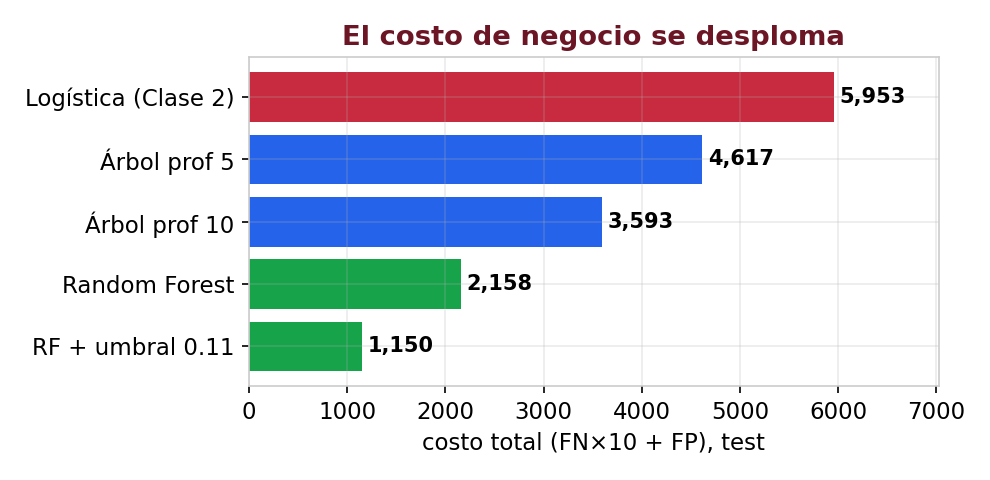
\includegraphics[width=\textwidth]{fig_costo_modelos.png}
    \end{column}
    \begin{column}{0.40\textwidth}
      {\footnotesize\color{textMuted}
      \begin{itemize}\setlength{\itemsep}{5pt}
        \item[{\color{codeGreen}\scriptsize\faCheck}]
          El bosque baja el costo de \textbf{5\,953 a 2\,158}:
          \textbf{64\,\% menos} que la logística.
        \item[{\color{codeGreen}\scriptsize\faTrophy}]
          Y aplicando el \textbf{umbral por costo} de la
          Clase 2: \textbf{1\,150}. Un \textbf{81\,\%} menos.
        \item[{\color{arcaRed}\scriptsize\faStar}]
          Zonas perdidas: de \textbf{563} (logística)
          a \textbf{42}.
      \end{itemize}
      }
    \end{column}
  \end{columns}

  \vspace{2pt}
  {\scriptsize\color{textMuted}
    \faLightbulb[regular]\hspace{3pt}%
    Las dos clases se suman: \textbf{mejor modelo} (hoy) \(\times\) \textbf{mejor decisión} (Clase 2).
    Ninguna reemplaza a la otra.}
\end{frame}

% ── IMPORTANCIA ──────────────────────────────────────────────────────────────
\begin{frame}{¿En Qué se Fija el Bosque?}
  \vspace{-6pt}
  {\small\color{arcaDark}\bfseries
    El bosque no da coeficientes, pero sí dice \textbf{cuánto usó} cada variable.}

  \vspace{4pt}
  \begin{columns}[T]
    \begin{column}{0.52\textwidth}
      \centering
      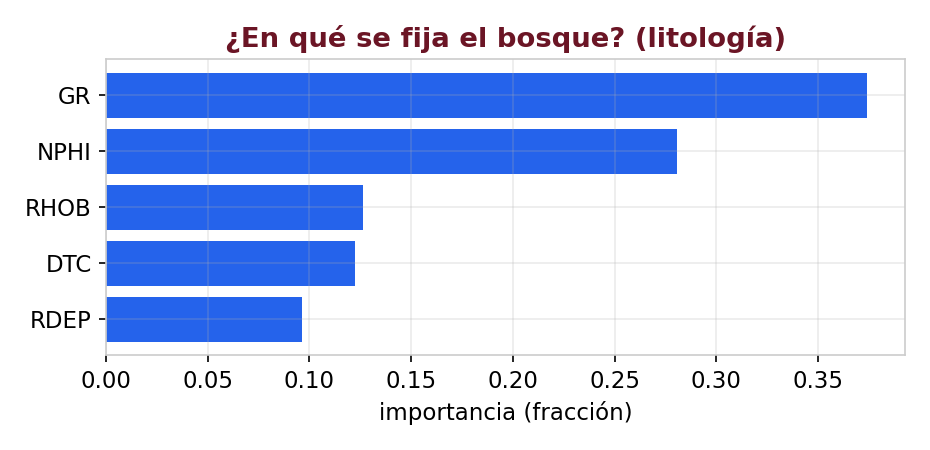
\includegraphics[width=\textwidth]{fig_importancia_lito.png}
    \end{column}
    \begin{column}{0.44\textwidth}
      {\footnotesize\color{textMuted}
      \begin{itemize}\setlength{\itemsep}{6pt}
        \item[{\color{codeGreen}\scriptsize\faTrophy}]
          \texttt{GR} domina (37\,\%) --- coherente con que
          el mejor corte univariado era GR = 49.
        \item[{\color{codeGreen}\scriptsize\faCheck}]
          \texttt{NPHI} segunda (28\,\%): la misma que el
          árbol pequeño eligió para refinar.
        \item[{\color{arcaRed}\scriptsize\faExclamationTriangle}]
          Ojo: importancia \(\neq\) causalidad. Dice qué
          \textbf{usó} el modelo, no qué \textbf{hace} que la
          roca sea arena.
      \end{itemize}
      }
    \end{column}
  \end{columns}
\end{frame}

% ── EL PRECIO ────────────────────────────────────────────────────────────────
\begin{frame}[shrink=10]{El Precio: Poder vs Explicabilidad}
  \vspace{-4pt}
  {\small\color{arcaDark}\bfseries
    Nada es gratis. Lo que ganamos en precisión lo pagamos en transparencia.}

  \vspace{6pt}
  \centering
  {\footnotesize
  \renewcommand{\arraystretch}{1.5}
  \begin{tabular}{@{}p{3.4cm} c c c@{}}
    \toprule
    & {\bfseries\color{arcaDark} Logística} & {\bfseries\color{arcaDark} Árbol} & {\bfseries\color{arcaDark} R.\ Forest} \\
    \midrule
    \rowcolor{arcaGray}
    Captura no linealidad & \color{arcaRed}no & \color{codeGreen}sí & \color{codeGreen}sí \\
    Resiste overfitting & \color{codeGreen}sí & \color{arcaRed}no & \color{codeGreen}sí \\
    \rowcolor{arcaGray}
    Se explica completo & \color{codeGreen}sí (fórmula) & \color{codeGreen}sí (diagrama) & \color{arcaRed}no (200 árboles) \\
    Necesita estandarizar & sí & no & no \\
    \bottomrule
  \end{tabular}
  }

  \vspace{8pt}
  {\footnotesize\color{textMuted}
  \begin{itemize}\setlength{\itemsep}{4pt}
    \item[{\color{arcaRed}\scriptsize\faArrowRight}]
      Del bosque solo podemos explicar las \textbf{importancias}, no el camino
      de cada predicción individual.
    \item[{\color{codeGreen}\scriptsize\faCheck}]
      La práctica profesional: \textbf{empezar simple} (línea base explicable) y
      \textbf{escalar} solo si el negocio necesita la precisión extra.
  \end{itemize}
  }
\end{frame}

% ── PRÁCTICA CLASIFICACIÓN ───────────────────────────────────────────────────
\begin{frame}[shrink=8]{Su Turno: Batir a la Logística \hfill {\normalsize\color{arcaRed}\faClock\hspace{4pt}15 min}}
  \vspace{-4pt}
  {\small\color{arcaDark}\bfseries
    En el notebook, con el dataset de litología ya cargado:}

  \vspace{6pt}
  {\footnotesize
  \begin{enumerate}\setlength{\itemsep}{6pt}
    \item[{\color{arcaRed}\bfseries 1.}]
      Entrenen un \texttt{DecisionTreeClassifier} con \texttt{max\_depth=3}.
      Grafíquenlo con \texttt{plot\_tree}: ¿qué preguntas eligió?
    \item[{\color{arcaRed}\bfseries 2.}]
      Prueben \texttt{max\_depth} = 2, 5, 10 y sin límite. Comparen accuracy
      en \textbf{train} y en \textbf{test}: ¿dónde empieza a memorizar?
    \item[{\color{arcaRed}\bfseries 3.}]
      Entrenen un \texttt{RandomForestClassifier} y saquen la \textbf{matriz de
      confusión}: ¿cuántas zonas perdidas quedaron?
    \item[{\color{arcaRed}\bfseries 4.}]
      Con \texttt{predict\_proba} y el costo de la Clase 2 (FN = 10\(\times\)FP),
      encuentren el \textbf{umbral óptimo} del bosque. ¿Baja de 2\,000?
  \end{enumerate}
  }
\end{frame}

% ═════════════════════════════════════════════════════════════════════════════
\sectionframe{Bonus: También Predicen Números}{Un medidor virtual de flujo}
% ═════════════════════════════════════════════════════════════════════════════

% ── EL PROBLEMA REGRESIÓN ────────────────────────────────────────────────────
\begin{frame}[shrink=8]{¿Cuánto Está Produciendo Cada Pozo, Ahora?}
  \vspace{-4pt}
  {\small\color{arcaDark}\bfseries
    Los árboles y bosques también hacen \textbf{regresión}. Un caso real para demostrarlo.}

  \vspace{6pt}
  \begin{columns}[T]
    \begin{column}{0.52\textwidth}
      {\footnotesize\color{textMuted}
      \begin{itemize}\setlength{\itemsep}{6pt}
        \item[{\color{arcaRed}\scriptsize\faFlask}]
          Medir el caudal de \textbf{un} pozo exige desviarlo al
          \textbf{separador de prueba}: se hace cada tantos días,
          no a diario.
        \item[{\color{arcaRed}\scriptsize\faBolt}]
          Lo que \textbf{sí} está siempre: los sensores de presión,
          temperatura y choke.
        \item[{\color{codeGreen}\scriptsize\faLightbulb}]
          \textbf{La idea}: estimar la producción desde esos
          sensores --- un \textit{medidor virtual de flujo}.
      \end{itemize}
      }
    \end{column}
    \begin{column}{0.44\textwidth}
      \begin{tcolorbox}[colback=arcaGray, colframe=arcaRed, boxrule=0pt, leftrule=3pt,
        arc=3pt, left=6pt, right=6pt, top=5pt, bottom=5pt]
        {\scriptsize\color{arcaDark}\bfseries El dataset (en el repo):}\\[4pt]
        {\scriptsize\color{textMuted}
          operación diaria de \textbf{5 pozos} de Volve:
          7\,862 días con \texttt{p\_fondo}, \texttt{p\_cabeza},
          \texttt{t\_cabeza}, \texttt{choke}, \texttt{dp\_choke},
          \texttt{horas} \(\to\) \texttt{oil} medido.}
      \end{tcolorbox}
      \vspace{4pt}
      {\scriptsize\color{textMuted}\itshape
        Los \textit{virtual flow meters} son un producto
        real de la industria.}
    \end{column}
  \end{columns}
\end{frame}

% ── LA CURVA + LA LINEAL CORTA ───────────────────────────────────────────────
\begin{frame}{Otra Vez la Física Curva}
  \vspace{-6pt}
  {\small\color{arcaDark}\bfseries
    La relación más fuerte (\texttt{p\_cabeza} vs \texttt{oil}) tiene forma de codo. La recta no puede.}

  \vspace{4pt}
  \begin{columns}[T]
    \begin{column}{0.54\textwidth}
      \centering
      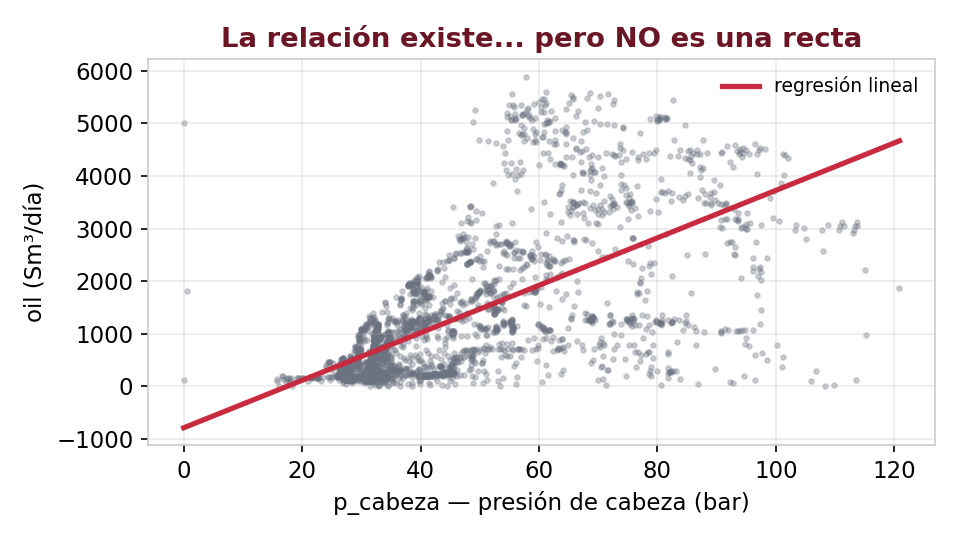
\includegraphics[width=\textwidth]{fig_curva_real.png}
    \end{column}
    \begin{column}{0.42\textwidth}
      {\footnotesize\color{textMuted}
      \begin{itemize}\setlength{\itemsep}{6pt}
        \item[{\color{arcaRed}\scriptsize\faTimes}]
          Regresión lineal con las 6 variables:
          R\textsuperscript{2} = \textbf{0.60}, error típico \textbf{583}
          Sm\(^3\)/día --- casi la mitad de la producción
          media (1\,264).
        \item[{\color{arcaRed}\scriptsize\faArrowRight}]
          No es que el problema sea impredecible:
          es que \textbf{la recta no dobla}.
      \end{itemize}
      }
    \end{column}
  \end{columns}
\end{frame}

% ── EL BOSQUE REGRESOR ───────────────────────────────────────────────────────
\begin{frame}{El Bosque Regresor: el Error se Desploma}
  \vspace{-6pt}
  {\small\color{arcaDark}\bfseries
    \texttt{RandomForestRegressor}: mismos árboles, pero cada hoja predice un \textbf{número} (el promedio de sus días).}

  \vspace{4pt}
  \begin{columns}[T]
    \begin{column}{0.54\textwidth}
      \centering
      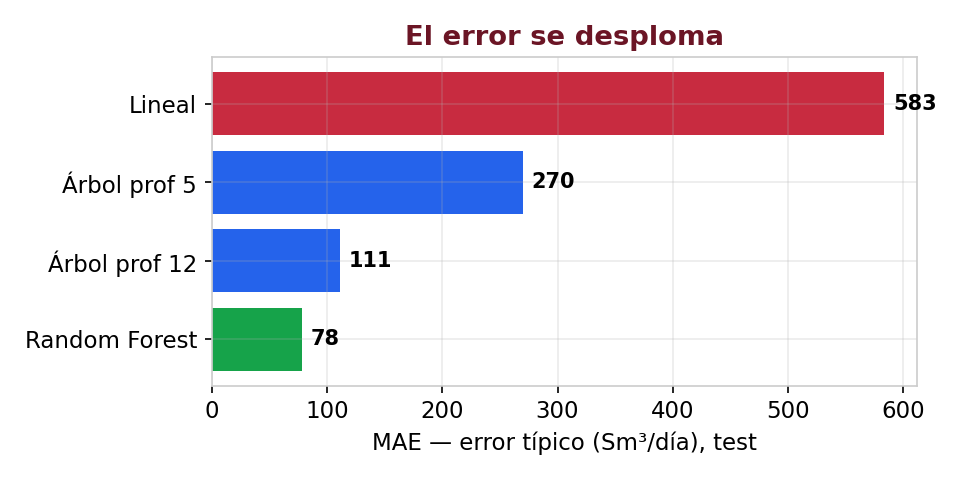
\includegraphics[width=\textwidth]{fig_comparacion.png}
    \end{column}
    \begin{column}{0.42\textwidth}
      {\footnotesize\color{textMuted}
      \begin{itemize}\setlength{\itemsep}{6pt}
        \item[{\color{codeGreen}\scriptsize\faCheck}]
          De \textbf{583} a \textbf{78} Sm\(^3\)/día de error:
          \textbf{7.5 veces menos}. R\textsuperscript{2} = 0.98.
        \item[{\color{codeGreen}\scriptsize\faCheck}]
          De inutilizable a \textbf{operativo}: el medidor
          virtual funciona.
        \item[{\color{arcaRed}\scriptsize\faArrowRight}]
          Y a diferencia de la recta del declive (Clase 1),
          el bosque \textbf{nunca predice producción
          negativa}: no inventa fuera de lo que vio.
      \end{itemize}
      }
    \end{column}
  \end{columns}
\end{frame}

% ── PRÁCTICA REGRESIÓN ───────────────────────────────────────────────────────
\begin{frame}[shrink=8]{Su Turno: el Medidor Virtual \hfill {\normalsize\color{arcaRed}\faClock\hspace{4pt}10 min}}
  \vspace{-4pt}
  {\small\color{arcaDark}\bfseries
    En el notebook, con el dataset de operación (\texttt{op}):}

  \vspace{6pt}
  {\footnotesize
  \begin{enumerate}\setlength{\itemsep}{6pt}
    \item[{\color{arcaRed}\bfseries 1.}]
      Exploren: scatter de \texttt{p\_cabeza} vs \texttt{oil}. ¿Ven el codo?
    \item[{\color{arcaRed}\bfseries 2.}]
      Entrenen la \textbf{regresión lineal} (línea base) y midan R\textsuperscript{2} y MAE en test.
    \item[{\color{arcaRed}\bfseries 3.}]
      Entrenen un \texttt{RandomForestRegressor} y comparen las mismas métricas.
    \item[{\color{arcaRed}\bfseries 4.}]
      Saquen las \textbf{importancias}: ¿qué sensor domina? ¿Tiene sentido físico?
    \item[{\color{arcaRed}\bfseries 5.}]
      Grafiquen \textbf{predicho vs real} del bosque en el test.
  \end{enumerate}
  }
\end{frame}

% ═════════════════════════════════════════════════════════════════════════════
\sectionframe{Cierre}{Lo que se llevan hoy}
% ═════════════════════════════════════════════════════════════════════════════

% ── RECAP ────────────────────────────────────────────────────────────────────
\begin{frame}[shrink=8]{Lo Que Aprendimos Hoy}
  \vspace{-4pt}
  \begin{columns}[T]
    \begin{column}{0.48\textwidth}
      {\footnotesize\color{arcaDark}\bfseries Conceptos}
      \vspace{3pt}
      {\footnotesize\color{textMuted}
      \begin{itemize}\setlength{\itemsep}{2pt}
        \item[{\color{codeGreen}\scriptsize\faCheck}]
          No linealidad: el paso deja de ser parejo
        \item[{\color{codeGreen}\scriptsize\faCheck}]
          La recta fracasa (las lunas)
        \item[{\color{codeGreen}\scriptsize\faCheck}]
          Árbol = preguntas encadenadas (raíz, hojas,
          profundidad)
        \item[{\color{codeGreen}\scriptsize\faCheck}]
          Cómo la máquina elige cada corte (pureza)
        \item[{\color{codeGreen}\scriptsize\faCheck}]
          Overfitting visible: train 1.000 vs test
        \item[{\color{codeGreen}\scriptsize\faCheck}]
          Random Forest: diversidad + voto
        \item[{\color{codeGreen}\scriptsize\faCheck}]
          Importancias (\(\neq\) causalidad); poder vs
          explicabilidad
      \end{itemize}
      }
    \end{column}
    \begin{column}{0.48\textwidth}
      {\footnotesize\color{arcaDark}\bfseries Herramientas}
      \vspace{3pt}
      {\footnotesize\color{textMuted}
      \begin{itemize}\setlength{\itemsep}{2pt}
        \item[{\color{arcaRed}\scriptsize\faTools}]
          \texttt{DecisionTreeClassifier} / \texttt{Regressor}
        \item[{\color{arcaRed}\scriptsize\faTools}]
          \texttt{RandomForestClassifier} / \texttt{Regressor}
        \item[{\color{arcaRed}\scriptsize\faTools}]
          \texttt{plot\_tree}, \texttt{feature\_importances\_}
        \item[{\color{arcaRed}\scriptsize\faTools}]
          \texttt{max\_depth}, \texttt{n\_estimators}
      \end{itemize}
      }
      \vspace{8pt}
      \begin{tcolorbox}[colback=arcaGray, colframe=arcaRed, boxrule=0pt, leftrule=3pt,
        arc=3pt, left=6pt, right=6pt, top=5pt, bottom=5pt]
        {\scriptsize\color{arcaDark}\bfseries El número del día:}\\[3pt]
        {\scriptsize\color{textMuted}
          costo de la litología: logística \textbf{5\,953}
          \(\to\) bosque + umbral \textbf{1\,150}.\\[2pt]
          \textbf{Mejor modelo} (hoy) \(\times\) \textbf{mejor decisión}
          (Clase 2).}
      \end{tcolorbox}
    \end{column}
  \end{columns}
\end{frame}

% ── PRÓXIMA ──────────────────────────────────────────────────────────────────
\begin{frame}{Lo Que Sigue}
  \vspace{-6pt}
  {\small\color{arcaDark}\bfseries
    Ya tienen modelos lineales y no lineales. Falta afinar cómo los validamos y ajustamos.}

  \vspace{10pt}
  {\footnotesize
  \begin{itemize}\setlength{\itemsep}{7pt}
    \item[{\color{arcaRed}\Large\faArrowCircleRight}]
      \textbf{Validación seria} --- validación cruzada, y el detalle que dejamos
      anotado: evaluar con \textbf{pozos completos} por fuera.

    \item[{\color{arcaRed}\Large\faArrowCircleRight}]
      \textbf{Afinar las perillas} --- búsqueda sistemática de hiperparámetros
      (\texttt{max\_depth}, \texttt{n\_estimators}\ldots).

    \item[{\color{arcaRed}\Large\faArrowCircleRight}]
      \textbf{Multiclase} --- las 11 litologías reales del FORCE 2020, con
      su matriz de penalización de la competencia.
  \end{itemize}
  }

  \vspace{10pt}
  \centering
  {\footnotesize\color{arcaDark}\itshape
    La pregunta de siempre sigue mandando: ¿qué decisión habilita este modelo
    y cuánto cuesta equivocarse?}
\end{frame}

% ── GRACIAS ──────────────────────────────────────────────────────────────────
\begingroup
\setbeamertemplate{headline}{}
\setbeamertemplate{footline}{}
\setbeamertemplate{navigation symbols}{}
\begin{frame}[plain, noframenumbering]
  \begin{tikzpicture}[remember picture, overlay]
    \fill[arcaDark] (current page.south west) rectangle (current page.north east);
    \node[anchor=center, text=white, font=\Huge\bfseries]
      at ([yshift=1.5cm]current page.center) {¡Gracias!};
    \node[anchor=center, text=white!80, font=\large, text width=10cm, align=center]
      at ([yshift=0.2cm]current page.center)
      {Carlos Enrique Mosquera Trujillo};
    \node[anchor=center, text=white!60, font=\normalsize, text width=10cm, align=center]
      at ([yshift=-0.6cm]current page.center)
      {\faEnvelope\hspace{6pt}cmosquerat@unal.edu.co};
    \node[anchor=center, text=white!60, font=\normalsize, text width=11cm, align=center]
      at ([yshift=-1.3cm]current page.center)
      {Machine Learning for Petroleum Engineers Using Python};
    \node[anchor=center, text=white!40, font=\small]
      at ([yshift=-2.0cm]current page.center)
      {SLB Ecuador \quad$\cdot$\quad UDLA \quad$\cdot$\quad 2026};
  \end{tikzpicture}
\end{frame}
\endgroup

\end{document}
